%%%% ijcai23.tex

\typeout{IJCAI--23 Instructions for Authors}

% These are the instructions for authors for IJCAI-23.

\documentclass{article}
\pdfpagewidth=8.5in
\pdfpageheight=11in

% The file ijcai23.sty is a copy from ijcai22.sty
% The file ijcai22.sty is NOT the same as previous years'
\usepackage{ijcai23}

% Use the postscript times font!
\usepackage{times}
\usepackage{soul}
\usepackage{url}
\usepackage[hidelinks]{hyperref}
\usepackage[utf8]{inputenc}
\usepackage[small]{caption}
\usepackage{graphicx}
\usepackage{amsmath}
\usepackage{amssymb}
\usepackage{amsthm}
\usepackage{booktabs}
\usepackage{algorithm}
\usepackage{algorithmic}
\usepackage[switch]{lineno}
\usepackage{multirow}


% Comment out this line in the camera-ready submission
\nolinenumbers

\urlstyle{same}

% the following package is optional:
%\usepackage{latexsym}

% See https://www.overleaf.com/learn/latex/theorems_and_proofs
% for a nice explanation of how to define new theorems, but keep
% in mind that the amsthm package is already included in this
% template and that you must *not* alter the styling.
\newtheorem{example}{Example}
\newtheorem{theorem}{Theorem}

% Following comment is from ijcai97-submit.tex:
% The preparation of these files was supported by Schlumberger Palo Alto
% Research, AT\&T Bell Laboratories, and Morgan Kaufmann Publishers.
% Shirley Jowell, of Morgan Kaufmann Publishers, and Peter F.
% Patel-Schneider, of AT\&T Bell Laboratories collaborated on their
% preparation.

% These instructions can be modified and used in other conferences as long
% as credit to the authors and supporting agencies is retained, this notice
% is not changed, and further modification or reuse is not restricted.
% Neither Shirley Jowell nor Peter F. Patel-Schneider can be listed as
% contacts for providing assistance without their prior permission.

% To use for other conferences, change references to files and the
% conference appropriate and use other authors, contacts, publishers, and
% organizations.
% Also change the deadline and address for returning papers and the length and
% page charge instructions.
% Put where the files are available in the appropriate places.


% PDF Info Is REQUIRED.
% Please **do not** include Title and Author information
\pdfinfo{
/TemplateVersion (IJCAI.2023.0)
}

\title{ACsleuth: Domain Adaptive and Fine-grained Anomalous Cell Detection for Single-cell Multiomics}


% Single author syntax
\author{
    Author Name
    \affiliations
    Affiliation
    \emails
    email@example.com
}

% Multiple author syntax (remove the single-author syntax above and the \iffalse ... \fi here)
\iffalse
\author{
First Author$^1$
\and
Second Author$^2$\and
Third Author$^{2,3}$\And
Fourth Author$^4$
\affiliations
$^1$First Affiliation\\
$^2$Second Affiliation\\
$^3$Third Affiliation\\
$^4$Fourth Affiliation
\emails
\{first, second\}@example.com,
third@other.example.com,
fourth@example.com
}
\fi

\begin{document}
\setlength{\parindent}{0pt}
\setlength{\parskip}{0pt}



\maketitle

\begin{abstract}
    Fined-grained anomaly detection at the cellular level is a crucial phase in diagnosing 
    conditions and pathological analyses. Since the single-cell RNA sequencing (scRNA-seq) 
    data analysis has been greatly prompted by the development of deep learning, we can 
    effectively detect anomalous cells and explore their detail types. However, most of 
    works simply focus on detecting anomalies within normal observations, overlooking the 
    opportunity for more detailed distinctions of them. Moreover, the essence of both 
    anomaly and fine-grained detection is to learn distinct representations for different 
    sample categories, suggesting a straightforward pipeline of sequentially detecting 
    anomalies then subtyping them. Thus, we introduce an innovative workflow called ACsleuth, 
    aiming at fine-grained Anomalous cell detection for single-cell multiomics, which 
    further contains a batch correction module to alleviate bias inherent in the raw 
    data. By employing a GAN model to reconstruct normal observations and leveraging the 
    reconstruction error as the assessment criterion for the anomaly detector, we then 
    utilize the DESC clustering method for scRNA-seq data to explore subtypes of anomalies. 
    Extensive experiments improve the superiority of ACsleuth both of the comparison with the 
    state-of-the-art anomaly detection methods in detecting anomalies and simple 
    combinations of anomaly detection and clustering methods in fine-grained anomalous detection tasks.
\end{abstract}

\section{Introduction}

Recently, single-cell RNA sequencing (scRNA-seq) technologies has developed rapidly, 
which allows us to better explore tissue heterogeneity at the cellular level. It yields 
a gene expression matrix, where each vector represents the expression values of specific 
genes across cells. In addition, detecting diseased cells, commonly referred to anomaly 
detection, constitutes a crucial phase in diagnosing conditions and conducting pathological 
analyses. Moreover, fine-grained detection of diseased cells, which can also be called subtyping, enables a more comprehensive 
understanding of disease classifications and facilitates the development of nuanced and 
efficacious treatment strategies. Therefore, leveraging the gene expression matrix derived 
from scRNA-seq empowers us to enhance detecting anomalous cells, then delve deeper into 
the exploration of their fine-grained subtypes.

Motivated by deep learning, previous studies for scRNA-seq data mainly focus on cell 
clustering and cell type annotation. The former aims to identify cell groups such as sczi-Desk \cite{sczi-Desk} 
and scCNC \cite{scCNC}, and the latter simply annotates these groups based on marker genes or another prior 
information such as ItClust \cite{ItClust}, scArches \cite{scArches}. 
However, both of aforementioned tasks are not ideally suited for fine-grained anomalous cells detection. 
Anomaly detection naturally exhibits class-imbalance characteristics, while the challenge 
in fine-grained anomaly detection lies in acquiring more precise representations of distinct cell types 
due to their inherent similarity. Nevertheless, employing reference-based methods can be challenging, given the presence of 
technical variation (e.g., different laboratory conditions) across diverse studies, 
commonly referred recognized as batch effects in molecular biology literature \cite{Polyphony}. 
The intricate nature of scRNA-seq data, characterized by noise, batch effects, high 
dimensionality and sparsity \cite{dands} poses challenges that impede these deep 
methods from achieving optimal performance directly based on the raw data.

Domain adaptation is a crucial consideration in biological data analysis. Under the same sequencing technique, one of most 
typical instances is correcting batch effect, as we have discussed above. For example, the gene expression of cells from 
the same tissue but obtained from different patients, may be interfered by pronounced batch effects. 
Additionally, data derived from different sequencing technologies exhibits heterogeneous distributions, while 
compared with scRNA-seq,other sequencing technologies like scATAC-seq are even rarer \cite{RNAmore}.
This dataset shift is commonly denoted as domain bias in computer vision, encompassing aspects 
such as style differences,diverse sensory devices, etc \cite{domainada}. Both batch effects within the same sequencing technique data and the bias arising from different 
sequencing technologies contribute to domain bias \cite{ACE}. However, most previous studies failed to 
recognize such shared characteristics between these two biases and tended to address them 
independently, which are neither elegant nor efficient.

Besides, most of anomaly detection studies work solely on identifying anomalies within normal 
observations, which often treating it as a class-imbalance binary classification task \cite{OA}. 
However, these studies overlook the opportunity for more detailed classification of 
anomalies, such as distinguishing between different types of tumors or various criminal 
behaviors. This limitation results in underutilization of the available data and hinders 
the ability to learn more granular representations of the anomalous observations. 
Furthermore, the core objective of both anomaly detection and fine-grained detection is to 
acquire a more nuanced representation for each type of samples. This shared optimalization 
goal suggests that these two tasks can seamlessly integrate into an entire pipeline. 
Starting with raw data encompassing both normal and anomalous samples, the pipeline can 
effectively distinguish anomalies of various subtypes.

To address these limitations, we propose an comprehensive workflow consists of fine-grained anomalous cell 
detection and batch correction for scRNA-seq data, named ACsleuth, aiming at 
subtyping anomalies from the raw data which contains various normal and diseased types of 
cells. Our contributions are summarized as follows:
\begin{itemize}

\item Methodologically, we introduce an innovative workflow called ACsleuth, which contains 
fine-grained anomalous cell detection. The anomaly detector is first trained 
unsupervisedly on the reference dataset which has only normal observations, then we learn 
the batch effects on the normal samples identified by the former detector and use it for 
the batch correction on anomaly sets sequentially, finally subtyping anomalies simply by a recent 
single-cell clustering method.
\item Innovatively, we achieve domain adaptation by tackling batch effects in the target dataset 
after removing anomalous observations and using datasets derived from different sequencing technologies 
as the reference and the target data. For the former, ACsleuth involves leveraging a wasserstein 
distance as the domain transfer loss in MMD, to learn the domain bias with solely normal cells 
then subsequently applying bias correction on the detected anomalies before fine-grained subtyping them. 
For the latter, we simply correct the domain bias in the cross-domain anomaly detection task to obtain 
distinct representations for anomalous cells.
\item Empirically, we conduct extensive experiments to validate the exceptional performance 
of ACsleuth. Across evaluations on three distinct scRNA-seq datasets and one scATAC-seq dataset 
for cross-domain anomaly detection task within different numbers of highly variable genes, 
ACsleuth consistently raised state-of-the-art in the majority of anomaly detection and 
fine-grained detection.
\end{itemize}
\section{Related Works}
\subsection{Anomaly Detection}
Anomaly detection usually relies on learning distinct representations between normal 
observations and anomalies. Many studies focus on representing normal observations and 
anomalies are detected by filtering representations that are dissimilar to normal ones. 
One straightforward manner is one-class classification, which aims to train a model that 
can accurately describe normal samples and then distinguish whether test samples are from 
the same distribution as the reference data. This kind of detectors is trained to learn a 
new representation \cite{RCA} \cite {liznerski} that 
enhances the dissimilarity between embeddings of normal and anomalous samples, thereby 
improving the detectability of anomalies. While the one-class assumption is vulnerable 
since real datasets often contain multiple inliers \cite{SLAD}.

Generative models are another standard procedure in detecting outliers. They learn by 
reconstructing normal observations, which leads to poor reconstruction of anomalies in 
the target data due to their distinct reconstruction error. This is attributed to the 
fact that the reference data for the anomaly detection task exclusively consists of 
normal observations.
Popular frameworks such as autoencoder (AE) \cite{odae}, generative adversarial 
networks \cite{GANad} are widely used. Nevertheless, such GAN-based 
models like \cite{EffGAN} still struggle with distinguishing multiple normal observations, and are prone to 
occurring model-collapse during training. Additionally, AE frameworks exhibit limitations 
handling the noisy or high-dimensional sparse data.
\subsection{Single Cell RNA-Seq Data Subtyping}
Single-cell subtyping aims to identify distinct subtypes within the same cell type, e.g., 
tumors, which is similar to a broader task called cell annotation. The essence of two 
tasks lies in learning representations that effectively capture the heterogeneity among 
distinct types to the fullest extent. Cell annotation simply follows three 
steps \cite{threestep}: learning a compact representation by projecting cells to a 
lower-dimensional space, mapping similar cells to groups in the low-dimensional 
representation (typically via clustering), and finally characterizing the differences in 
gene expression among the cell groups. ACE \cite{ACE} uses AE to generate 
low-dimensional representations and considers the intrinsic dependencies among genes. 
Kratos \cite{kratos} fuses the dimension reduction and clustering cells to 
optimize jointly. scTAG \cite{scTAG} simultaneously identifies cells clusters and 
learns topological representations between cells. scPOT \cite{scPOT} achieves 
annotating seen cell types and novel cell type clustering simultaneously. For subtype 
detection, SCEVAN \cite{SCEVAN} and CopyKAT \cite{CopyKAT} are designed 
specifically for tumors since they used the prior information, CAMLU \cite{CAMLU} 
exhibits a higher degree of generality via the employment of AE, albeit its performance is suboptimal. 

Detecting subtypes solely involves assigning labels to distinct types of observations, 
while cell annotation demands the utilization of prior information to assign specific 
labels to the cells. However, compared to cell annotation, subtype detection necessitates 
the acquisition of more robust representations. Given that the observations from different 
subtypes fall under the same subcategory, the inherent differences between them tend to 
be subtler. Therefore, fine-grained subtype detection relies heavily on distinctive representations to 
achieve accurate classification. In summary, both anomaly detection and fine-grained detection 
necessitate learning precise representations, so that it is straightforward that we can 
propose a pipeline comprising anomaly detection and fine-grained subtype detection via the identical objective. 
Notably, to the best of our knowledge, none of the previous works are designed for a 
comprehensive workflow which contains such subtasks including anomaly detection and 
anomalies detailed multi-classification.
\begin{figure}
    \centering
    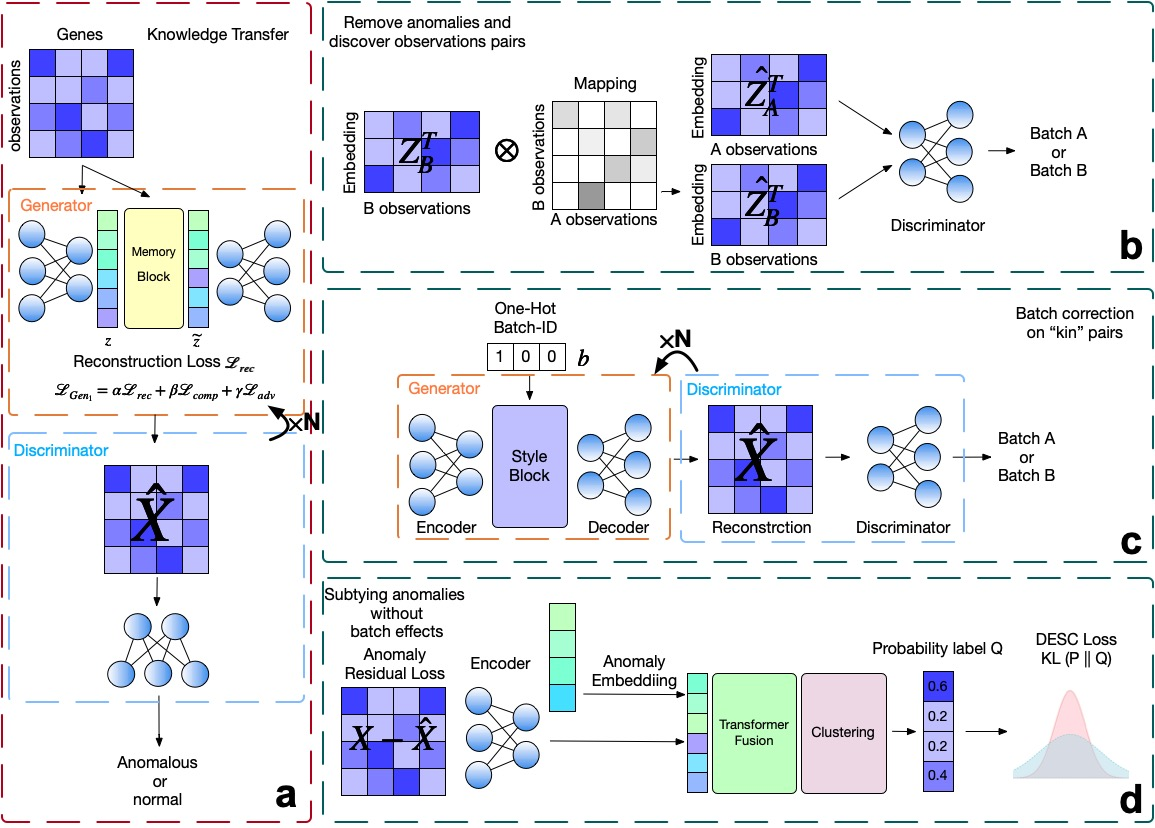
\includegraphics[scale=0.20]{Framework.jpg}
    \caption{Illustration of ACSleuth. The overall model consists of GAN-based anomaly detection and batch effect correction modules and DESC clustering module for fine-grained anomalous cell detection.}
\end{figure} 
\section{Methods}
We first give an overview of subtyping cells workflow, which can be divided into two main 
parts: anomaly detection and subtype clustering. We start with training the detector 
unsupervisedly, as the reference dataset contains only normal cells. The target dataset 
contains two kinds of labels: the two-class one for distinguishing between normal and 
anomalous cells, and the detailed one for categorizing subtypes of cells. Specifically, 
we exclusively leverage the subtyping module for anomalies discovered by the detector, 
which we refer to as “pre-anomalies”. That means they may include a few “fake anomalies”. 
Finally, we use true anomalies and their detailed labels to evaluate the effects of 
subtyping, since we solely focus on anomalies’ subtypes instead of considering normal 
cells. Then we combine it with the former detector to fully assess the whole pipeline. 
ACsleuth consists of three modules, each dedicated to anomaly detection, batch effect correction and subtyping.
\subsection{Detecting Anonaly Cells}
ACsleuth detects anomalies based on learning the reconstruction of normal 
observations from the reference dataset through the generative adversarial networks (GAN). 
As the GAN model is specifically trained to reconstruct solely normal observations, 
anomalous cells in target datasets are more likely to hold larger reconstruction errors, 
which are treated as an assessment criterion for the detector.
Our GAN module (referred as \textit{module I}) simply consists of a generator and a discriminator. 
The generator can be subdivided into three distinct components: an encoder, a decoder and 
a memory block. Instead of random weights initialization, we choose to pretrain the encoder 
and the decoder on auxiliary datasets for the pre-text task focused on data reconstruction, 
which alleviates the model degeneration. Let $x_i$ denote the gene expression vectors of the cell 
$i$ in scRNA-seq, the architectural backbone of the encoder is a MLP network. Thus, we have 
the embeddings of the cell $i$ from:
\begin{equation}
    z_i = f_{\textit{MLP}}(x_i)
\end{equation}
The memory block is fundamentally an embedding queue $Q\in\mathbb{R}^{N_{mem}\times p}$ 
filled with $z_i\in\mathbb{R}^p$, as $N_{mem}$ is defined as the number of in-memory 
embeddings. It is initialized with embeddings generated by the pretrained encoder and 
provides an attention-based 
means for reconstructing the embedding as $\widetilde{z} \in \mathbb{R}^p$: 
\begin{equation}
    \widetilde{z}_i = Q^T \mathbf{softmax}\left(\frac{Qz_i}{\tau}\right)
\end{equation}
where $\tau$ is the temperature hyperparameter. During the entire training procedure,  
$Q$ is dynamically updated by enqueuing the most recently 
reconstructed $\widetilde{z}$ and dequeuing the oldest ones, thereby striking 
a balance between preserving learnt features and adapting to new observations, and also 
effectively mitigating the risks of mode collapse. The decoder then reconstructs $x_i$ from 
the transcriptomic embeddings $\widetilde{z_\mathbf{i}}$. Decoders for 
generating $\widehat{x_i}$ are also implemented using MLP-based, since the simpler 
architectures improve both model efficiency and flexibility without compromising the 
overall performance \cite{AGC}. Besides, $\widehat{x_i}$ passes the same encoders 
to generate $\widehat{z_i}$ for calculating comparative loss between the original and re-encoded embeddings.

The discriminator $D$ is trained to distinguish whether x and $\hat{x}$ is real or 
generated data. Therefore, loss functions of the generator and the discriminator for 
anomaly detection is defined as:
\begin{equation}
\begin{split}
    \mathcal{L}_{\text{Gen}_1} &= \alpha\mathcal{L}_{\text{rec}} + \beta\mathcal{L}_{\text{comp}} + \gamma\mathcal{L}_{\text{adv}} \\
    &= \alpha\mathbb{E}{||x - \widehat{x}||}_1 + \beta\mathbb{E}{||z - \widehat{z}||}_2 - \gamma\mathbb{E}[D(\widehat{x})] \\
\end{split}
\end{equation}
\begin{equation}
    \mathcal{L}_{D_1} = \mathbb{E}\left[D\left(\widehat{x}\right)\right] - \mathbb{E}\left[D\left(x\right)\right] + \lambda\mathbb{E}[{({||\nabla D (\widetilde{x})^2||}_2 - 1)}^2]  
\end{equation}
where $\ \widetilde{x}=\epsilon\widehat{x}_i+\left(1-\epsilon\right){x},\ \epsilon\in\left(0,1\right)$. 
$\mathcal{L}_{rec}$ 
is defined as the data reconstruction loss, $\mathcal{L}_{comp}$ denotes the comparative 
loss between the original and the re-encoded embeddings. $\mathcal{L}_{adv}$ denotes the 
adversarial loss. $\alpha, \beta, \gamma\geq0$ represent the weights of three loss functions. 
$D\left(\widehat{x}_i\right)$ represents the probability of classifying  $\widehat{x}_i$ as 
the real observation. Significantly, the discriminator’s loss function contains of a 
gradient penalty factor, which promotes the stability of the adversarial training and 
reduces the risk of mode collapse \cite{wGANs}.
Once the training is completed, ACsleuth is leveraged to reconstruct observations from target 
scRNA-seq or scATAC-seq datasets. We define the anomalous score as the cosine 
dissimilarity between embeddings of the original and the reconstructed observations to 
assess the reconstruction accuracy of an observation $i$:
\begin{equation}
    d_i = 1-\frac{{z_i}^T\widehat{z}_i}{||{z_i}^T||\cdot||\widehat{z}_i||}
\end{equation}
A higher $d_i$ refers to a lower reconstruction accuracy, which means the 
observation $i$ is more likely to be anomalous. Lastly, we give a predefined threshold to 
detect outliers based on those anomalous scores that exceed the specified limit.

\textbf{Cross-domain Anomaly Detection.}	Based on transfer learning, we train the 
detector to reconstruct normal observations within the reference scRNA-seq dataset 
and simply apply it on the target scATAC-seq dataset. While the former focuses on gene 
expression, the latter reveals cell’s chromatin accessibility, both data domains capture 
single-cell information, which can be regarded as different views of the same single cell. 
As they have the identical data structures, this cross-domain task shows ACsleuth is capable 
of learning a robust representation of the entire cell thereby exhibiting strong 
generalization performance.
\subsection{Multi Sample Batch Effect Correction}
The identification and removal of confounding anomalies from target datasets empower 
ACsleuth to align multiple target datasets onto the feature space of the reference dataset, 
thus fulfilling the task of multi-sample batch correction for single-cell data. As 
illustrated in figure 1, this task contains two subtasks: (1) matching each normal sample 
in the target datasets with its most analogous counterpart in the reference dataset. A 
pair of such samples is termed a “kin” pair, indicating that the two paired samples are 
more likely to share identical biological contents. (2) learning a “style-divergence” 
matrix to represent the batch effects between target datasets and the reference dataset. 
This matrix can then be applied to map target datasets to the reference data space in a 
“style-transfer” manner.

Formally, we first define the batch effect in the context of gene expression analysis as: 
\begin{equation}
    x_{ij}={x_{ij}}^{'}+b_j+\epsilon_{ij}
\end{equation}
where $x_{ij}$ denotes the gene expression values for $j-th$ cell in the batch $i$, $b_{ij}$ 
is the batch effects of the batch $i$ and the term $\epsilon_{ij}~N(0,1)$ represents random noise, 
which is uneffected by batch effects.

For the first subtask, we introduce a GAN module (referred as \textit{module II}) that takes 
as input the embeddings of normal observations from both the reference and target datasets, 
which are generated by the encoder within \textit{module I}. The generator of this module is 
trained to learn a non-negative mapping matrix for generating observations in target 
datasets through those in the reference dataset, while the discriminator corresponding to 
learning to distinguish the authentic and generated observations. In detail, let $N_T$ 
and $N_R$ denote the number of observations in the target and reference dataset, then 
define $Z_T\in\mathbb{R}^{N_T\times p}$ as the embeddings of multi-sample target datasets, 
$Z_R\in\mathbb{R}^{N_R\times p}$ the embeddings of the reference dataset, 
$M\in\mathbb{R}^{N_T\times N_R}$ the trainable non-negative mapping matrix. The generated 
observation represents as: 
\begin{equation}
    {\widehat{Z}}_T=ReLU(M)Z_R 
\end{equation}
The rectified linear unit (ReLU) function serves as the non-negative constraint on $M$. 
Furthermore, we indicate the loss functions for the generator and the discriminator of 
\textit{module II} as:
\begin{equation}
    \mathcal{L}_{\text{Gen}_2} = \alpha\mathbb{E}\|Z_T - \widehat{Z}_T\|_1 - \beta\mathbb{E}[D(\widehat{Z}_T)] 
\end{equation}
\begin{equation}
        \mathcal{L}_{D_2} = D(\widehat{Z}_T) - \mathbb{E}\left[D(Z_T)\right] + \lambda\mathbb{E}\left[({\|\nabla D(\widetilde{Z}_T)\|}_2 - 1)^2\right]
\end{equation}
where  $\widetilde{Z}=\epsilon\widehat{Z}+\left(1-\epsilon\right)Z,\ 
\epsilon\in\left(0,1\right)$.$\alpha,\beta,\lambda\geq0$ represent the weights of the loss 
terms. Upon the completion of the adversarial training of \textit{module II}, the column index of 
the maximum value on the $i^{th}$ row of matrix M corresponds to the index of the reference 
observation that forms a “kin” pair with the $i^{th}$ observation in the target dataset. 
We propose a hypothesis that observations belonging to the same “kin” pair share analogous 
biological content, allowing us to approximate the reference observation by eliminating 
the “style-divergence” from the target observation. Therefore, for the second subtask, a 
GAN for “style-transfer” (referred as \textit{module III}) is employed to learn the 
“style-divergences”, or namely batch effects, between pairs of the target and reference 
datasets as rows of a trainable matrix $S\in\mathbb{R}^{N_{batch}\times p}$ in the latent 
embedding space. In detail, for an observation i in the target datasets, the encoder of 
the generator within \textit{module III} maps its raw gene expression vector 
$x_i$ to $z_i\in\mathbb{R}^p$ in the latent embedding space. This latent representation is 
then employed to estimate the embeddings of its “kin” observation $j$ as follows:
\begin{equation}
z_i=f_{\textit{MLP}}(x_i,W_5), {\widehat{z}}_j = z_i-S^T b_i
\end{equation}
where $b_i\in\mathbb{R}^{N_{batch}}$ denotes {i}’s one-hot encoded batch-identity vector for 
selecting the corresponding “style-divergence” row from $S$. In sequence, the decoder of the 
generator maps ${\hat{z}}_j$ back to the original reference data space as ${\hat{x}}_j$. The 
discriminator of \textit{module III} is simply trained to distinguish the $x_j$ and ${\hat{x}}_j$. We 
indicate the loss functions for the generator and the discriminator of \textit{module III} as:
\begin{equation}
\mathcal{L}_{Gen_3}=\alpha\mathbb{E}{||x_R- \widehat{x}_R||}_1-\beta\mathbb{E}[D(\widehat{x}_R)]
\end{equation}
\begin{equation}
\mathcal{L}_{D_3}=\mathbb{E}\left[D\left(\widehat{x}_R\right)\right]-\mathbb{E}\left[D\left(x_R\right)\right]+\lambda\mathbb{E}[{({||\nabla D(\widetilde{x}_R)||}_2-1)}^2]
\end{equation}
where $\alpha,\beta,\lambda$ and $\widetilde{x}_R$ have the same definitions as 
their counterparts in \textit{module II}. Finally, observations in multiple target datasets can be 
batch-corrected and aligned in the common reference data space by passing through the 
trained generator within \textit{module III}.
\subsection{Fine-grained Anomalous Cell Detection}
\begin{table}
    \centering
    \begin{tabular}{cccccc}
        \hline
        DATA  & Type & Genes  & Cells & Anomaly Ratio \\
        \hline
        \multirow{2}{*}{\centering PBMCs} & \multirow{2}{*}{\centering scRNA-seq} & \multirow{2}{*}{\centering 32738}  & 3684 & 13.14\%  \\
        & & & 3253 & 12.73\% \\ 
        \multirow{2}{*}{\centering Cancer} & \multirow{2}{*}{\centering scRNA-seq} & \multirow{2}{*}{\centering 33538} & 7721 & 50.03\%  \\
        & & & 4950 & 58.12\% \\ 
        TME & scATAC-seq & 23127 & 2968 & 60.24\% \\
        \hline
    \end{tabular}
    \caption{Information of Datasets.}
    \label{tab:plain}
\end{table}


In this section, we introduce how ACsleuth subtypes anomaly cells detected by preceding 
modules. Since \textit{module III} can align anomalies identified by module I across multiple 
target datasets in the common reference space, thus significantly mitigating the 
confounding batch variations and facilitating the anomaly subtyping task. Specifically, we 
combine the embeddings and reconstruction loss generated by \textit{module I} to distinguish 
between various novel cell subtypes and address the variations among them. We first give 
some notations: for an anomalous cell $i$, ${x_i}^g$ denotes 
cell’s batch-corrected gene expression vector, and 
${\widehat{x}_i}^g$ the gene expression vector reconstructed by 
\textit{module I}, respectively. ${r_i}^g$ represents the reconstruction 
loss of gene expressions. $z_i$ and $\zeta_i$ represent the embeddings of 
$x_i$ and $r_i$, which are also generated by the 
encoder within \textit{module I}. Above terms are calculated as follows:
\begin{equation}
{r_i}^g = {x_i}^g-{{\widehat{x}}_i}^g, r_i = {r_i}^g
\end{equation}
\begin{equation}
    \begin{split}
        z_i = f_{\textit{MLP}}({x_i}^g,W_1),{z_i}^\ast = TF([z_i||\zeta_i],W_{tf}), 
    \end{split}
\end{equation}
\[
   where \zeta_i = f_{\textit{MLP}}({r_i}^g,W_1)    
\]
where ${z_i}^\ast$ represents the fused embeddings and reconstruction 
loss of anomalous cell $i$ by a transformer fusion (TF) block. We then leverage a 
discriminatively boosted clustering algorithm, DESC \cite{DESC}, to cluster 
anomalies according to their  $z^\ast$. In detail, DESC applies a Cauchy kernel 
to compute the soft assignment score of an anomaly cell i to a cluster $j$ as:
\begin{equation}
    q_{i,j} = \frac{{{(1 + \left\| z_i^\ast - \mu_j \right\|^2 / v)}}^{-1}}{{\sum_{j'} \left(1 + \left\| z_i^\ast - \mu_{j'} \right\|^2 / v\right)^{-1}}}
\end{equation}
where $q_{i,j}$ represents the probability that cell $i$ belongs to cluster $j
, \mu_j$ the centroid of cluster $j, v$ the degree of freedom of the Cauchy kernel. 
The clustering loss function is a KL-divergence $\mathcal{L}$ calculated on $q$ and an 
auxiliary target distribution $p$, defined as:
\begin{equation}
p_{i,j}=\frac{q_{i,j}^2/\sum_{i} q_{i,j}}{\sum_{j}\left(q_{i,j}^2/\sum_{i} q_{i,j}\right)} 
\end{equation}
\begin{equation}
    \mathcal{L}=\sum_{i}{\sum_{j} p_{i,j}log\left(\frac{p_{i,j}}{q_{i,j}}\right)}
\end{equation}
Note that anomalies with a high-confident assignment are overweighted in p. 
Experimentally, the iterative updating of TF weights $W_{TF}$ and cluster 
centroid $\mu$ with the objective of minimizing $\mathcal{L}$ drives q to p, 
resulting in a gradual transformation of harder-to-cluster embeddings 
$z^\ast$ into easier ones. The self-paced and iterative DESC persists until the 
change in the hard assignments of anomalous cells falls below a predefined threshold or 
reaches a predefined number of iterations. The subtype labels of anomalies can be readily 
obtained from their final hard cluster assignments. Additionally, the number of subtype 
labels is assumed to beknown or automatically inferred during the clustering. In detail, 
\section{Experiments}
\begin{table*}
    \centering
    \resizebox{\textwidth}{!}{
    \begin{tabular}{cccccccccc}
        \hline
        DATA & Anomaly & Highly Genes & ACsleuth & SLAD & ICL & NeuTraL & RCA & AE & Scmap \\
        \hline
        \multirow{6}{*}{\centering PBMCs} & \multirow{3}{*}{\centering B Cells} & 3000 & \textbf{0.833$\pm$0.034} & 0.347$\pm$0.023 & 0.262$\pm$0.029 &0.299$\pm$0.014 & 0.267$\pm$0.007 & 0.449$\pm$0.015 & 0.377$\pm$0. \\
        & & 6000 & \textbf{0.818$\pm$0047} & 0.279$\pm$0.021 & 0.246$\pm$0.024 & 0.234$\pm$0.022 & 0.266$\pm$0.009 & 0.401$\pm$0.008 & 0.393$\pm$0. \\
        & & full & \textbf{0.785$\pm$0.044} & 0.149$\pm$0.007 & 0.176$\pm$0.014 & 0.215$\pm$0.010 & 0.266$\pm$0.006 & 0.258$\pm$0.006 & 0.390$\pm$0. \\
        & \multirow{3}{*}{\centering NK Cells} & 3000 & \textbf{0.804$\pm$0.004} & 0.548$\pm$0.013 & 0.307$\pm$0.042 & 0.330$\pm$0.025 & 0.258$\pm$0.025 & 0.462$\pm$0.012 & 0.495$\pm$0. \\
        & & 6000 & \textbf{0.819$\pm$0.022} & 0.587$\pm$0.021 & 0.359$\pm$0.038 & 0.351$\pm$0.030 & 0.259$\pm$0.024 & 0.545$\pm$0.006 & 0.615$\pm$0. \\
        & & full & \textbf{0.757$\pm$0.035} & 0.607$\pm$0.015 & 0.168$\pm$0.013 & 0.294$\pm$0.065 & 0.259$\pm$0.024 & 0.617$\pm$0.005 & 0.589$\pm$0. \\ 
        \hline
        \multirow{6}{*}{\centering Cancer} & \multirow{3}{*}{\centering Epithelial \& Immune Tumor} & 3000 & \textbf{0.926$\pm$0.009} & 0.881$\pm$0.006 & 0.856$\pm$0.006 & 0.889$\pm$0.011 & 0.818$\pm$0.033 & 0.896$\pm$0.002 & 0.679$\pm$0. \\
        & & 6000 & 0.832$\pm$0.014 & \textbf{0.862$\pm$0.004} & 0.844$\pm$0.005 & 0.847$\pm$0.006 & 0.600$\pm$0.041 & 0.853$\pm$0.003 & 0.683$\pm$0. \\
        & & full & \textbf{0.826$\pm$0.035} & 0.785$\pm$0.005 & 0.572$\pm$0.006 & 0.691$\pm$0.040 & 0.649$\pm$0.009 & 0.717$\pm$0.006 & 0.734$\pm$0. \\
        & \multirow{3}{*}{\centering Epithelial \& Stromal Tumor} & 3000 & 0.860$\pm$0.049 & 0.888$\pm$0.014 & 0.899$\pm$0.018 & \textbf{0.913$\pm$0.008} & 0.677$\pm$0.036 & 0.746$\pm$0.005 & 0.688$\pm$0. \\
        & & 6000 & 0.824$\pm$0.007 & 0.828$\pm$0.014 & 0.856$\pm$0.014 & \textbf{0.892$\pm$0.008} & 0.543$\pm$0.025 & 0.681$\pm$0.006 & 0.735$\pm$0. \\
        & & full & \textbf{0.717$\pm$0.059} & 0.638$\pm$0.005 & 0.556$\pm$0.006 & 0.686$\pm$0.024 & 0.471$\pm$0.026 & 0.571$\pm$0.003 & 0.683$\pm$0. \\
        \hline
        \multirow{3}{*}{\centering TME} & \multirow{3}{*}{\centering Tumor(pre)} & 3000 & & 0.582$\pm$0.011 & 0.791$\pm$0.050 & 0.578$\pm$0.016 & 0.493$\pm$0.030 & 0.488$\pm$0.001 & 0.752$\pm$0. \\
        & & 6000 & & 0.590$\pm$0.017 & 0.728$\pm$0.028 & 0.591$\pm$0.013 & 0.511$\pm$0.038 & 0.509$\pm$0.002 & 0.733$\pm$0. \\
        & & full & & 0.640$\pm$0.021 & 0.756$\pm$0.012 & 0.638$\pm$0.017 & 0.538$\pm$0.032 & 0.532$\pm$0.002 & 0.529$\pm$0. \\
        \hline
        \multirow{3}{*}{\centering PBMC-TME} & \multirow{3}{*}{\centering Tumor(pre)} & 3000 & & 0.570$\pm$0.021 & 0.583$\pm$0.032 & 0.645$\pm$0.044 & 0.$\pm$0. & 0.524$\pm$0.002 & 0.$\pm$0.  \\
        & & 6000 & & 0.573$\pm$0.034 & 0.629$\pm$0.044 & 0.637$\pm$0.070 & 0.$\pm$0. & 0.533$\pm$0.001 & 0.$\pm$0. \\
        & & full & & 0.562$\pm$0.019 & 0.637$\pm$0.031 & 0.664$\pm$0.054 & 0.$\pm$0. & 0.524$\pm$0.001 & 0.$\pm$0. \\
        \hline
    \end{tabular}
    }
    \caption{Average F1 score with standard deviation for anomaly detection on single-cell transcriptomics datasets.}
    \label{tab:plain}
\end{table*}

\begin{table*}
    \centering
    \resizebox{\textwidth}{!}{
    \begin{tabular}{ccccccccc}
        \hline
        DATA  & Anomaly & Highly Genes & ACsleuth & DFCN & EDESC & scTAG & Leiden & K-Means \\
        \hline
        \multirow{6}{*}{\centering Cancer} & \multirow{3}{*}{\centering Epithelial \& Immune Tumor} & 3000 & \textbf{0.926$\pm$0.009} & 0.881$\pm$0.006 & 0.856$\pm$0.006 & 0.889$\pm$0.011 & 0.818$\pm$0.033 & 0.896$\pm$0.002 \\
        & & 6000 & 0.832$\pm$0.014 & \textbf{0.862$\pm$0.004} & 0.844$\pm$0.005 & 0.847$\pm$0.006 & 0.600$\pm$0.041 & 0.853$\pm$0.003 \\
        & & full & \textbf{0.826$\pm$0.035} & 0.785$\pm$0.005 & 0.572$\pm$0.006 & 0.691$\pm$0.040 & 0.649$\pm$0.009 & 0.717$\pm$0.006 \\
        & \multirow{3}{*}{\centering Epithelial \& Stromal Tumor} & 3000 & 0.860$\pm$0.049 & 0.888$\pm$0.014 & 0.899$\pm$0.018 & \textbf{0.913$\pm$0.008} & 0.677$\pm$0.036 & 0.746$\pm$0.005 \\
        & & 6000 & 0.824$\pm$0.007 & 0.828$\pm$0.014 & 0.856$\pm$0.014 & \textbf{0.892$\pm$0.008} & 0.543$\pm$0.025 & 0.681$\pm$0.006 \\
        & & full & \textbf{0.717$\pm$0.059} & 0.638$\pm$0.005 & 0.556$\pm$0.006 & 0.686$\pm$0.024 & 0.471$\pm$0.026 & 0.571$\pm$0.003 \\
        \hline
    \end{tabular}
    }
    \caption{Average F1*NMI score with standard deviation for fine-grained anomaly detection on single-cell transcriptomics datasets.}
    \label{tab:plain}
\end{table*}
\subsection{Experimental Settings}
\textbf{Dataset.}	Our experiments contain anomaly cells’ detection and anomaly cell 
clustering. Furthermore, each task splits to two parts. For the former, we use datasets 
simply called PBMCs, Cancer and TME, including scRNA-seq and scATAC-seq, as we have both 
intra-data detection and cross-data detection. In detail, we specifically treat B cells 
and natural killer (NK) cells as anomalies in PBMCs. For the latter, we use Cancer for 
the task of single-batch and concatenate different batches for the multi-batch task. The 
detailed information is described in Table 1. Each dataset is split according to the 
number of highly variable genes, including 3000, 6000 and all genes respectively. Besides, 
we normalize and log the data using the Scanpy \cite{scanpy} package.

\textbf{Baselines.} For the anomaly detection, we compare ACsleuth with four recently 
state-of-the-art anomaly detection methods in tabular data (SLAD \cite{SLAD}, 
ICL \cite{ICL}, NeuTraL \cite{NeuTraL}, RCA \cite{RCA}) and two 
classical methods (Scmap \cite{scmap} and AE \cite{AE}). The code 
we use is provided by authors, and each one we use default hyperparameters if no specific 
instructions are given.

For the fine-grained anomalous cell detection, we compare ACsleuth with the combination of one baseline of 
anomaly detection and the state-of-the-art method of clustering. The former we choose the 
SLAD, as it has better performance both in the ability of both detecting anomalies and 
computational efficiency than other baselines. Then select four recent clustering methods 
(scTAG \cite{scTAG}, EDESC \cite{EDESC}, DFCN \cite{DFCN}, Leiden \cite{leiden} 
and K-means \cite{kmeans}), including deep embedded clustering and scRNA-seq 
clustering, and one classical clustering method. 

\textbf{Evaluation Metrics.}	We assess the performance with two widely used evaluation metrics: 
F1 score for anomaly detection, normalized mutual information (NMI) for cell clustering. 
For the cell’s subtype detection, we simply multiply the F1 score and the NMI to create 
a new metric, which is used to measure the effect of the whole task. The higher the values 
of these metrics, the better the detecting and the clustering performance. The reported 
metrics are averaged results with standard deviations over ten independent runs.

\textbf{Implementation Details.} 	Our experiments are conducted with a 
NVIDIA GeForce RTX 3090 GPU and 24GB of memory.  (Hyperparameters settings)

\subsection{Results}
\textbf{Anomaly detection results.}	Table 1 illustrates the detection performance in terms of 
F1 score, of our model ACsleuth and the competing methods. Each dataset’s best detector is 
boldfaced. On the three datasets with different number of highly variable genes, we totally 

\textbf{Anomaly detection Cross-domain results.}	To evaluate the generalization capacity of ACsleuth 
in anomaly detection, we trained the model on the PBMCs then tested it on the TME. The 
former dataset is the scRNA-seq data, while the latter is the scATAC-seq data, both 
representing different domains for the same cells. Specifically, we screen out genes 
common to both datasets, then still split them according to the number of highly variable 
genes. The performance of ACsleuth and baseline methods illustrate in the bottom of Table 1. Results 
demonstrate that ACsleuth outperforms baseline anomaly detection methods, which means it can 
construct robust representations for each single-cell.

\textbf{Anomalies fine-grained detection results.}	We evaluate ACsleuth by comparing it with simple combinations 
of anomaly detection methods and clustering methods for the fine-grained anomaly detection task. In 
this section, we assess the impact of fine-grained detection task in two scenarios: the 
single-batch representing a common condition and multi-batch where different batches of 
Cancer datasets are concatenated to emphasize the importance of batch effect correction 
in scRNA-seq data. As shown in Table 2, we can conclude that for the single-batch task, 
ACsleuth consistently achieves stable and superior performance, as reflected by the product 
of F1 scores for detecting anomalies and NMI scores for clustering on most of cases. In 
the multi-batch task, ACsleuth significantly outperforms baseline methods. Results fully 
demonstrate that batch effects are intractable for recent methods. ACsleuth addresses this 
challenge by learning such kind of biases from the normal observations split from anomaly 
detection, then subsequently correcting them on the detected anomalies before subtyping 
them. We empirically establish the necessity of the batch correction module for the scRNA-seq data analysis.

\textbf{Computational Performance.}
\subsection{Ablation Studies}
In this section, we conduct a series of ablation studies to validate how different 
configurations of each module impact the anomaly subtyping task. We still assess ACsleuth with 
the Cancer dataset since it contains more genes (features) and cells (observations). We 
present experiments sequentially for anomaly detection, batch effect correction and anomaly 
subtyping as outlined below.

\textbf{Effect of memory bank for anomaly detection.}	As introduced in section 3.1, 
we employ a memory block to enhance the training of the anomaly detector. In particular, 
we evaluate ACsleuth without the memory block in the anomaly detection module, and results are 
illustrated in Figure 2. Upon the removal of the memory block, the anomaly detection 
module easily collapses, significantly impairing affect the subsequent subtyping task.

\textbf{Essence of the batch correction module.}	We have discussed that batch effect correction 
is imperative for the scRNA-seq data analysis. It is straightforward to question whether 
the subtyping results will be worse if we directly subtype anomalies observations after 
detecting them, following the same settings as baseline methods. As shown in figure 2, 
the direct connection of two tasks is considerably adverse compared with the original ACsleuth.

\textbf{Validity of the reconstruction error in the fine-grained detection task.}	At last, we carry out an 
ablation study for the input of the fine-grained anomaly detection module. The 
reconstruction error generated from anomaly detection module (\textit{Module I}) serves as 
anomalous scores leveraged to identify anomalies in \textit{Module I}, encompassing similarity 
information among them. If we merely consider the original gene expression matrix as the 
input of subtype clustering, there will be an underutilization of information regarding 
anomalous cells, as empirically demonstrated in figure 2.
\section{Conclusion}
In this paper, we innovatively propose ACsleuth, a comprehensive workflow that sequentially 
integrates anomaly detection with fine-grained anomaly detection, which further contains a batch 
correction module to alleviate bias inherent in the raw data. More precisely, we first 
employ a GAN-based model to detect anomalies according to the reconstruction error, then 
capture batch effects from filtered normal observations and correct them on the detected 
anomalies. We also prove that the domain adaptation module is effective for cross-domain tasks. 
Finally, we utilize the DESC clustering algorithm to fine-grained detecting anomalous cells. 
ACsleuth outperforms state-of-the-art approaches in anomaly detection methods for tabular 
data and their simple combinations with deep clustering algorithms. Empirically results 
strongly improve ACsleuth’ superiority, demonstrating its generalizability and robustness. 
We’d like to further explore the potential of the domain adapyative fine-grained anomaly 
detection workflow for tabular data generalized to another fields.
\section*{Acknowledgments}



%% The file named.bst is a bibliography style file for BibTeX 0.99c
\bibliographystyle{named}
\bibliography{ijcai23}

\end{document}

